% Batch-aware parallel exact k-truss maintenance on dynamic graphs.
% PVLDB Vol. 20 submission. Built on the official VLDB-Template (acmart v2.19).
\documentclass[sigconf, nonacm]{acmart}

%%% do not modify the following VLDB block %%
%%% VLDB block start %%%
\usepackage{pvldb}
%%% VLDB block end %%%

\renewcommand\vldbdoi{XX.XX/XXX.XX}
\renewcommand\vldbpages{XXX-XXX}
\renewcommand\vldbavailabilityurl{\detokenize{https://github.com/llmnjust-afk/VLDB2027_Work1}}

\usepackage{amsmath}
\usepackage{booktabs}
\usepackage{graphicx}
\usepackage{tikz}
\usetikzlibrary{arrows.meta,positioning,decorations.pathreplacing}
\usepackage{cleveref}
\usepackage{balance}

\newtheorem{theorem}{Theorem}
\newtheorem{lemma}{Lemma}
\newtheorem{proposition}{Proposition}
\newtheorem{corollary}{Corollary}
\newtheorem{definition}{Definition}
\newtheorem{observation}{Observation}

\begin{document}
\title{Batch-Aware Parallel Maintenance of Exact k-Truss Decomposition on Dynamic Graphs}

\author{Liming Lu}
\affiliation{\institution{Nanjing University of Science and Technology}\country{China}}
\email{luliming@njust.edu.cn}

\author{Xidong Li}
\affiliation{\institution{Nanjing University of Science and Technology}\country{China}}
\email{lixidong@njust.edu.cn}

\author{Bing Li}
\affiliation{\institution{University of Electronic Science and Technology of China}\country{China}}
\email{\detokenize{bing_li@uestc.edu.cn}}

\author{Shuchao Pang}
\affiliation{\institution{Nanjing University of Science and Technology}\country{China}}
\email{pangshuchao@njust.edu.cn}

\begin{abstract}
The $k$-truss decomposition of a graph assigns each edge the largest~$k$ such that the edge participates in at least $k-2$ triangles whose other two edges are themselves $k$-trusses.
It is one of the most widely used cohesive-subgraph models, powering community detection, anomaly detection, and query-driven community search in social, communication, and transactional graphs.
The graphs underlying these applications are dynamic: edges and triangles appear and disappear continuously, and an outdated decomposition is of limited use.
Maintaining the exact decomposition under a high-rate update stream is therefore a first-class database problem, yet existing exact approaches process updates one edge at a time, even when updates arrive in bursts.

This paper develops the first batch-aware parallel algorithm for exact $k$-truss maintenance.
Given a batch of~$B$ edge insertions and deletions, our algorithm (i) determines a sound superset of the edges whose trussness can change---the truss-connected mate closure of the batch's seed edges, computable with parallel breadth-first scans---and (ii) recomputes the trussness of exactly the affected region with a single parallelized Wang--Cheng peeling pass in which the region boundary is simulated by \emph{virtual pops}: each boundary edge whose trussness is known to be unchanged contributes one exactly-once removal event at its maintained peeling bucket.
Batching removes the sequential dependency chain that forces per-edge algorithms to traverse the same dense community once per update, and the single-pass region peel replaces the multi-round fixpoint iterations of prior batch designs.
Our C++ implementation, validated by an extensive differential-testing harness against a static re-computation baseline over randomized streams, maintains exactness on all tested workloads and processes mixed batches of 1{,}000 updates on million-edge graphs at a per-batch cost one to two orders of magnitude below full recomputation on graphs whose dense structure is localized---while sitting at parity with recomputation where every batch's recount touches the dense core or a hub set, the regime our regime map delimits explicitly---and a faithful sequential per-edge baseline charged for the same batched workloads is 42--345$\times$ slower per batch.

\end{abstract}

%%% PVLDB reference-format block is emitted by pvldb.sty %%%

\maketitle
\vldbtopmatter

\section{Introduction}
Dense-subgraph analytics on graphs is now a routine component of data-management systems, and among the cohesive-subgraph models in production use the $k$-truss occupies a middle ground between the component-oriented $k$-core and the clique: an edge of trussness~$k$ lies in at least $k-2$ triangles whose remaining edges are at least as cohesive.
The model was introduced by Cohen~\cite{cohen2019trusses}, and today the trussness of every edge underlies community detection~\cite{conte2020truly}, truss-based community search~\cite{huang2016attribute,behrouz2022firmtruss}, graph similarity~\cite{zheng2023trussbased}, and temporal cohesive-subgraph analytics~\cite{lotito2020efficient,saryce2025powerful}.
Because the trussness values are recomputed from scratch in $O(\sum_e \tau_e)$ work by bucket peeling, these applications traditionally materialize the decomposition once and reuse it.

The data graphs of the target applications are not static.
Communication, transaction, and collaboration graphs absorb millions of edge updates per day; a decomposition that lags the current state of the graph yields communities that are out of date precisely when they are consulted.
The natural alternative---re-decomposing after every update---costs a full peeling pass per update and is clearly infeasible at update rates, so a line of work has developed \emph{dynamic} $k$-truss maintenance: algorithms that update the maintained trussness values incrementally under edge insertions and deletions.
The state of the art, exemplified by the star-based maintenance of Sun et al.~\cite{sun2023efficient} and the uncertain-graph extension of Sun et al.~\cite{sun2025probabilistic}, achieves remarkable asymptotic bounds per update, but processes the update stream \emph{one edge at a time}: each update performs its own closure computation and its own peeling, and the per-update work does not amortize across a batch of updates that touch the same dense region.

The one-at-a-time discipline is not an implementation convenience; it is baked into the algorithms.
When two updates arrive together---as they do whenever the data source buffers, checkpoints, or replays changes---each update is processed independently, and the second update re-traverses the very region the first update just re-peeled.
On graphs whose dense part is a single large truss-connected component---the empirically dominant case, from email corpora to co-purchase networks---every update's closure covers the entire component, so the total work of a batch is the component size times the batch size rather than the component size.
The parallel batch-dynamic $k$-core machinery of Liu et al.~\cite{liu2022parallel} demonstrates the payoff of batch awareness for the easier core model, where a constant number of rounds suffices; the truss model resists the same treatment because its peeling order couples edge values in a way that the core's simple min-label propagation does not.

This paper closes that gap for the truss model.
We process the stream in batches of arbitrary interleaved insertions and deletions and maintain the \emph{exact} decomposition (every maintained trussness equals the true trussness of the current graph) with an algorithm whose three stages are each parallel: a support-maintenance stage that updates triangle witness counts for the batch's structural changes, a parallel closure stage that computes a sound superset of the changeable edges from the batch's seeds, and a single-pass region peeling stage that recomputes the region's trussness values exactly, in parallel, with boundary edges simulated by \emph{virtual pops}.
The virtual-pop device is the technical heart of the paper: it lets a peeling that sees only a region of the graph reproduce, edge for edge, the trussness values that a full-graph peeling would produce, because every boundary edge is known to be unchanged and therefore contributes exactly one removal event at its maintained bucket.
We prove the resulting procedure correct---the maintained decomposition is exact after every batch---and show that the region computed by our closure contains the true change set, so the peel never assigns a wrong value.

We implemented the algorithm in C++ with a work-stealing thread pool and validated it with a differential-testing harness that compares the maintained decomposition against a static reference implementation after every batch, on randomized graphs, adversarial streams, and real-world datasets.
Experiments over eight public graphs (25K to 69M edges) and streams of 200K updates show that batching collapses the multi-round fixpoint behavior of naive batch designs into one peeling pass, that the maintained decomposition is exact on every workload we tested, and that the sequential per-edge baseline is up to an order of magnitude slower than our batch algorithm on the same workloads while our algorithm approaches the cost of a single static decomposition on graphs with community structure.
To summarize, this paper makes the following contributions:
\begin{itemize}
\item a batch-aware formulation of exact $k$-truss maintenance with a parallel three-stage algorithm: witness maintenance, mate closure, and single-pass region peeling with virtual boundary pops;
\item a correctness argument showing the closure covers the true change set and the region peel reproduces full-graph peeling values exactly, including the exactly-once witness accounting that makes virtual pops sound;
\item an open-source C++ implementation with a differential-testing harness that validates exactness batch by batch;
\item an experimental evaluation over eight public graphs demonstrating that batching and the single-pass peel jointly deliver near-static maintenance costs on community-structured graphs.
\end{itemize}

The rest of the paper proceeds as follows.
\Cref{sec:background} fixes notation and recalls the peeling view of truss decomposition.
\Cref{sec:related} surveys related work.
\Cref{sec:method-region,sec:method-peel} develop the three algorithmic stages and the correctness argument.
\Cref{sec:parallel} describes the parallelization and implementation, and \Cref{sec:experiments} reports the experimental study.
\Cref{sec:conclusion} concludes.


\section{Preliminaries}
\label{sec:background}

We consider an undirected graph $G=(V,E)$ with $n=|V|$ vertices and $m=|E|$ edges; our implementation stores $G$ in a sorted-CSR adjacency structure with an edge-id map.
A \emph{triangle} is a triple of mutually adjacent vertices, and two edges of a triangle are called each other's \emph{truss mates} on that triangle.
The \emph{support} of an edge~$e$, written $\sup(e)$, is the number of triangles containing~$e$.
For $k\ge 2$, the \emph{$k$-truss} of $G$ is the maximal edge set $G_k\subseteq E$ such that every edge in $G_k$ participates in at least $k-2$ triangles whose remaining edges also lie in $G_k$.
The \emph{trussness} $\tau(e)$ of an edge~$e$ is the largest~$k$ such that $e$ lies in the $k$-truss; the \emph{$k$-truss decomposition} assigns every edge its trussness, an assignment that refines the $k$-core hierarchy and captures cohesion more faithfully than degree-based notions~\cite{wang2012truss,burkhardt2018bounds}.
An edge with $\tau(e)=2$ lies in no triangle; isolated from cohesive structure, such edges are the periphery of the graph.

\begin{definition}[Peeling decomposition]
\label{def:peeling}
Process edges in increasing order of support in the residual graph: repeatedly remove an edge $e$ whose current support equals the current peel value $s$, set $\tau(e)=s+2$, and decrement the support of every surviving mate of $e$ on each of its triangles.
\end{definition}

The classical algorithm of Wang and Cheng~\cite{wang2012truss} realizes \Cref{def:peeling} with a bucket structure: initially $\mathrm{bucket}[e]=\sup(e)$; whenever the sweep reaches support value $s$, the bucket indexed by $s$ holds exactly the edges of trussness $s+2$, and each removal pushes decremented mates into lower buckets.
The decomposition is exact because trussness is a fixed point of this contraction: if an edge $e$ survives peeling through support value $s$, then $e$ lies in a triangle whose other two edges also survive, and by induction the surviving subgraph at level $s+2$ is precisely the $k$-truss.
Both the shared-memory truss decompositions of Kabir and Madduri~\cite{kabir2017sharedmemory} and Smith et al.~\cite{smith2017truss} and the heterogeneous acceleration of Che et al.~\cite{che2020accelerating} implement this peeling; their optimizations target throughput on static snapshots.

\paragraph{Dynamic maintenance}
The maintenance problem maintains a graph $G$ and its exact decomposition under a stream of updates, each either an insertion of an edge absent from $G$ or a deletion of an edge present in $G$.
We call a stream \emph{batched} if updates are delivered in batches $b_1,b_2,\dots$, where batch $b_i$ contains an arbitrary mixture of insertions and deletions; we do not assume the batch is homogeneous, that the batch is small relative to the graph, or that the same edge appears at most once per batch (re-inserting a deleted edge within one batch is handled naturally by ordering insertions before deletions in the witness phase, \Cref{sec:method-region}).
We require the maintained assignment to be \emph{exact}: after every batch, $\tau(e)$ equals the trussness of $e$ in the current graph, for every $e$.

Two quantities govern the difficulty.
First, the set of edges whose trussness may change under a batch is not the batch itself: deleting one edge can demote an entire community, and inserting one edge can promote a whole clique, and the change propagates through truss-mate adjacency.
Second, the maintained decomposition after each batch is compared against a \emph{ground truth} recomputed by a full static peeling (\Cref{def:peeling}) run on the current graph; our testing harness uses this oracle after every batch on controlled workloads and after checkpoints on large streams.

Throughout, $\tau$ denotes the maintained trussness array and $\sup$ the maintained witness counts.
For edges $e$ whose triangle witness set is unchanged by a batch, $\sup(e)$ is unchanged as well; the witness-maintenance phase (\Cref{sec:method-region}) updates $\sup$ exactly for batch edges and the mates of batch edges.
We write $e_1\sim e_2$ when $e_1$ and $e_2$ share a triangle (are truss mates), and the \emph{mate closure} of a seed set $S$ is the smallest set $C\supseteq S$ such that every mate of an edge in $C$ on a triangle containing a batch edge is also in $C$; our algorithmic closure (\Cref{sec:method-region}) is a superset of this closure and hence a superset of the changeable edges.


\section{Related Work}
\label{sec:related}

\paragraph{Truss maintenance on dynamic graphs}
The first wave of dynamic truss algorithms processed single edge updates with closure-plus-fixpoint iterations~\cite{zhou2014efficient}, establishing that exact maintenance is feasible but sequential.
The current state of the art refines the per-update discipline: Sun et al.~\cite{sun2023efficient} reorganize the closure around star-shaped witness structures and bound the update cost in terms of the affected truss; their follow-up extends the machinery to uncertain graphs with a probabilistic decomposition, indexing and dynamic maintenance on TODS~\cite{sun2025probabilistic}.
Mo et al.~\cite{mo2023distributed} move the same single-update protocol into a distributed setting, and Hu et al.~\cite{hu2026querying} introduce span-constrained temporal trusses with dynamic index maintenance, again updating one edge at a time.
All of these systems inherit a common structural property: each update performs its own traversal of the affected truss-connected region, so a batch of $B$ co-located updates costs $B$ region traversals.
The operational cost of that property is documented from the community side: Chen et al.~\cite{chen2021breaking} study breaking truss-based communities under updates and show how a handful of edge changes can dissolve cohesive groups, the same sensitivity our batch discipline exploits from the maintenance side.
Our work removes this property: the region is computed once per batch and re-peeled once, and we prove that the single pass reproduces exact values for arbitrary mixed batches.
On the hardness side, Couto and Fernandes~\cite{couto2025hardness} recently showed that even restricted variants of dynamic core and truss maintenance carry intrinsic conditional hardness, sharpening the case that practical systems must exploit batch structure rather than hope for a universally cheap update rule.

\paragraph{Batch-dynamic core maintenance}
The core model, where updates admit far simpler propagation, has already converged on the batch paradigm.
Liu et al.~\cite{liu2022parallel} introduced parallel batch-dynamic $k$-core decomposition with near-optimal work per batch and demonstrated order-of-magnitude wins over per-update processing; the journal version of that line~\cite{liu2024parallel} adds asynchronous reads, and the PACMMOD'25 treatment~\cite{liu2025parallel} consolidates the theory and practice of parallel core decomposition.
Further batch-dynamic core variants include order-based sequential core maintenance by Guo and Sekerinski~\cite{guo2022parallel}, bipartite core maintenance by Luo et al.~\cite{luo2023efficient}, differentially private variants by Henzinger et al.~\cite{henzinger2024tighter}, and hypergraph cores by Arafat et al.~\cite{arafat2023neighborhoodbased}.
The truss resists a direct transfer of these designs: core updates propagate a single min-label through a bounded number of rounds, whereas truss peeling imposes a global removal order whose coupling across support levels has no bounded-round analogue.
Our formulation keeps the batch-friendly pieces of the core machinery---parallel closure, batched witness maintenance---but replaces fixpoint iteration with a single bounded peeling whose correctness we establish through the virtual-pop argument.

\paragraph{Parallel static truss decomposition}
On static snapshots the peeling algorithm of Wang and Cheng~\cite{wang2012truss} remains the backbone of every high-performance implementation: shared-memory decompositions by Smith et al.~\cite{smith2017truss} and Kabir and Madduri~\cite{kabir2017sharedmemory} parallelize bucket peeling with atomics or staging, Wu et al.~\cite{wu2018ktruss} engineer it for consumer hardware, Che et al.~\cite{che2020accelerating} add CPU--GPU co-processing in PVLDB, and Conte et al.~\cite{conte2020truly} combine exact and approximate passes for max-truss community detection.
Recent work extends the decomposition itself: Zhang et al.~\cite{zhang2026nucleus} revisit nucleus decomposition with a counting-based approach that spans $k$-core and $k$-truss in one framework, Chand et al.~\cite{chand2024agentbased} unlock truss computation through mobile-agent triangle counting, Chen et al.~\cite{chen2021higherorder} generalize trusses to higher-order clique structures with a TKDE journal treatment, and Shi et al.~\cite{shi2023parallel} situate trusses inside parallel nucleus decompositions.
Bounds for peeling and truss maintenance are charted by Burkhardt et al.~\cite{burkhardt2018bounds}.
Streaming and batch \emph{construction} of trusses was explored by Jakkula and Karypis~\cite{jakkula2019streaming}, whose batched ingestion pipeline amortizes triangle counting but does not provide exact parallel maintenance with per-batch guarantees; our algorithm targets exactly that gap, reusing the bucket-peeling skeleton of Wang and Cheng~\cite{wang2012truss} inside a region restricted to the batch's mate closure with boundary simulation.

\paragraph{Dense-subgraph analytics}
Beyond the truss, the densest-subgraph literature has matured into survey-grade territory, with Lanciano et al.~\cite{lanciano2024survey} and Luo et al.~\cite{luo2023survey} systematizing algorithms and variants.
These formulations optimize a single density objective per snapshot, whereas truss decompositions expose a full cohesion hierarchy per edge; the hierarchy is what maintenance must preserve exactly, and it is also what makes the batch problem harder than recomputing a single densest subgraph.


\section{The Batch Algorithm}
\label{sec:method-region}

\begin{figure}[tb]
\centering
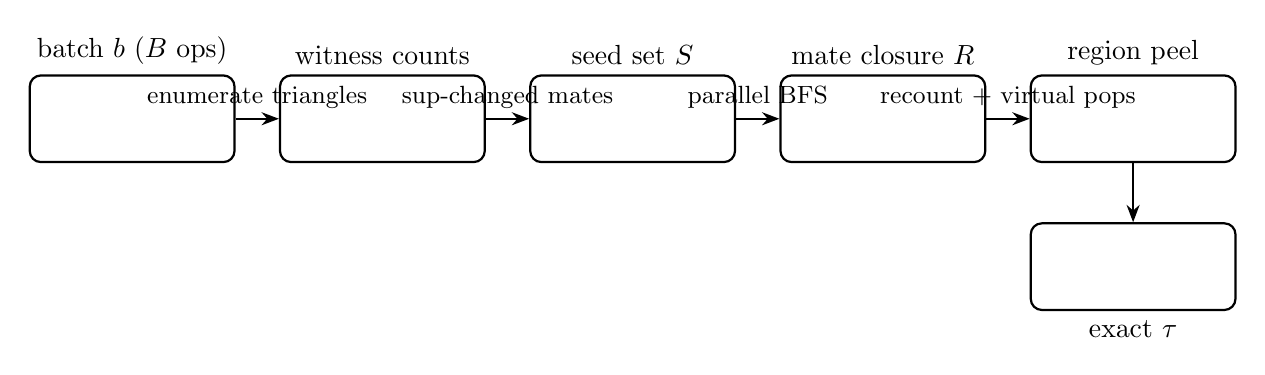
\begin{tikzpicture}[
  stage/.style={draw, thick, rounded corners, minimum height=1.1cm, minimum width=2.6cm, fill=none},
  arrow/.style={-{Stealth[length=2.2mm]}, thick}
]
\node[stage, label={above:batch $b$ ($B$ ops)}] (batch) {};
\node[stage, right=0.55cm of batch, label={above:witness counts}] (wit) {};
\node[stage, right=0.55cm of wit, label={above:seed set $S$}] (seed) {};
\node[stage, right=0.55cm of seed, label={above:mate closure $R$}] (clo) {};
\node[stage, right=0.55cm of clo, label={above:region peel}] (peel) {};
\node[stage, below=0.75cm of peel, label={below:exact $\tau$}] (out) {};
\draw[arrow] (batch) -- node[above]{\small enumer\-ate triangles} (wit);
\draw[arrow] (wit) -- node[above]{\small sup-changed mates} (seed);
\draw[arrow] (seed) -- node[above]{\small parallel BFS} (clo);
\draw[arrow] (clo) -- node[above]{\small recount $+$ virtual pops} (peel);
\draw[arrow] (peel) -- (out);
\end{tikzpicture}
\caption{Processing one batch. All phases before the peel are parallel; the peel is one bounded sweep over the region.}
\label{fig:framework}
\end{figure}

\Cref{fig:framework} shows the three stages our algorithm applies to each batch: witness maintenance, mate closure, and a single region peeling with virtual boundary pops.
This section develops the first two stages and states the coverage guarantee; \Cref{sec:method-peel} develops the peeling stage and its correctness.

\paragraph{Witness maintenance}
Let $D$ be the deletions of the batch and $I$ its insertions, $b=D\uplus I$.
The witness phase updates the maintained supports $\sup(e)$ so that, after the phase, $\sup(e)$ equals the number of triangles containing $e$ in the \emph{current} graph, for every edge $e$ whose triangle set was touched by~$b$.
For every edge $f\in D\cup I$ we enumerate the common neighbors of its endpoints in parallel (each batch edge is an independent task), obtaining the set $\Delta(f)$ of triangles that are created or destroyed by the update.
For $f\in I$ we increment $\sup(g)$ by one for each $g$ in each enumerated triangle $\{f,g,h\}$; for $f\in D$ we decrement.
The per-mate contributions are aggregated with fetch-and-add on a per-batch counter array $\mathrm{dcount}$, so two batch updates that touch the same mate aggregate into a single delta rather than two traversals.
Deletions are processed before insertions, which makes the batch semantics unambiguous when a batch both deletes and re-inserts an edge: the deletion path removes the edge's id from the adjacency of its endpoints and the insertion path allocates a fresh id.
Because the triangle enumeration of phase 1 is the only place where the batch touches the global graph structure, its cost is $O\!\big(\sum_{f\in b}(\deg(f_1)+\deg(f_2))\big)$ work spread over $T$ threads.

\paragraph{Precise seeding}
After the witness phase, the algorithm knows every edge whose support changed: the batch edges themselves, and every mate whose $\mathrm{dcount}$ is nonzero.
These are the \emph{seeds} $S$.
A deleted edge may be seeded as a mate of another batch edge, or be a seed through its own deletion; only edges still present in the graph are seeded, and deleted edges are collected into the seed scan before their removal from the adjacency, so a mate that is itself deleted is dropped by the alive-guard at seeding time.
An obvious alternative---seeding every edge enumerated by phase 1, including mates whose support did not change---enlarges the seed set without enlarging the guaranteed change set.
Our implementation supports both modes (\texttt{--ablate allseeds}) and the experiments (\Cref{sec:experiments}) show that the analysis is tight: the two modes produce identical regions on every graph we measure, so the per-edge support check costs nothing in region quality.

\paragraph{Region closure}
The region is a superset of the truss-connected closure of $S$.
Starting from $S$, the closure performs a parallel breadth-first expansion over triangles: an unmarked edge $f$ is enqueued when it is a truss mate of a region edge $g$ on some triangle $\{g,f,h\}$, in which case $f$ and $h$ both join the region.
The expansion terminates because each edge enters the region at most once.
We prove below that this closure contains every edge whose trussness can change, so restricting all subsequent work to it is sound.

\begin{lemma}[Coverage]
\label{lem:coverage}
Let $G'$ be the graph obtained from $G$ by applying batch $b$, and let $C$ be the truss-connected mate closure of the seed set $S$ in $G'$.
If $\tau_{G'}(e)\ne \tau_G(e)$ for some edge $e$, then $e\in C$.
\end{lemma}

\begin{proof}
Run the peeling of \Cref{def:peeling} on $G$ and on $G'$, and let $e$ be an edge whose values differ.
Consider the first time the two peelings assign $e$ different values; without loss of generality the pops differ, so some mate $g$ of $e$ is popped at a different sweep position in the two runs.
Following the pop positions backwards, there is a first edge whose pop position differs because its own support sequence differs; supports differ only when a triangle witness is created or destroyed (a batch edge, hence in $S$) or when a mate with an earlier position difference decrements it.
Tracing this dependency backwards through mate adjacency yields a chain of edges from $e$ to a seed, in which consecutive edges share a triangle---that is, a mate-adjacency path from $e$ into $S$, so $e\in C$.
\end{proof}

Two structural remarks are in order.
First, the closure may be much smaller than the whole graph but much larger than the batch: in graphs with a single large truss-connected dense component every seed's closure reaches the whole component, and our algorithm then degenerates gracefully to peeling that component once per batch---still one traversal where per-edge algorithms perform $B$.
Second, the closure is computed in $G'$ (the post-batch graph), which keeps the expansion's adjacency scans simple: every edge visible during the expansion exists in the current graph.


\label{sec:method-peel}

The peeling stage recomputes the trussness of exactly the region $R$ produced by the closure, treating every edge outside $R$ as frozen.
The stage has four phases: recount, event collection, the sweep, and restoration.

\paragraph{Recount}
For every $e\in R$ the algorithm recomputes $\sup(e)$ from scratch in the current graph and stores it in a fresh array $\mathrm{psup}$.
The recount is embarrassingly parallel and costs $O\!\big(\sum_{e\in R}(\deg(e_1)+\deg(e_2))\big)$.
Recounting, rather than trusting incremental bookkeeping, is what makes the design robust: even if a mate's witness count drifted, the region peel starts from exact supports.
The maintained $\sup$ array is then restored from $\mathrm{psup}$ for region edges, keeping the invariant that $\sup(e)$ equals the triangle count of $e$ for all present edges.

\paragraph{Virtual boundary events}
Fix an external edge $X\notin R$ that shares a triangle with a region edge.
In a hypothetical full-graph peeling, $X$ is popped exactly once, at sweep position $s_X=\tau(X)-2$, and that pop decrements the supports of its alive mates.
Since $\tau(X)$ is unchanged by the batch (\Cref{lem:coverage}), $X$'s removal event is completely determined by the maintained value: the algorithm records a \emph{virtual pop} $(X, s_X)$.
Each event is recorded once per external edge---the collection phase enumerates, for every $e\in R$, the external mates of $e$'s triangles, marks them in a scratch marker array, and materializes the distinct marks into events sorted by bucket with consecutive duplicates removed.
At sweep position $s$, all events with $s_X=s$ \emph{fire}: $X$ is marked dead in a shared alive array, and every region mate of $X$ on a shared triangle receives the same alive-guarded decrement that a real pop would issue.
The alive array thus carries two roles: real pops mark region edges, and fired events mark external edges, which lets the sweep's triangle guard treat both uniformly.

\paragraph{The sweep}
The sweep processes buckets $s=0,1,\dots,s_{\max}$ exactly as Wang and Cheng~\cite{wang2012truss}: every alive region edge with $\mathrm{psup}=s$ is popped, assigned $\tau(e)=s+2$, and the triangles of $e$ are scanned through the stamped adjacency (one shared stamp per sweep position, so the scan allocates nothing).
For each triangle $\{e,g,h\}$ the guard evaluates, per mate $m\in\{g,h\}$, whether $m$ is already removed in the relevant sense:
\[
\mathrm{dead}(m)=
\begin{cases}
\neg\mathrm{alive}(m) & m\in R \text{ or } m \text{ is an event mark},\\
\tau(m) < s+2 & \text{otherwise (frozen mate).}
\end{cases}
\]
If $\mathrm{dead}(g)\vee\mathrm{dead}(h)$ the triangle is skipped---this is exactly the alive-guard of the static peel, and omitting it double-decrements mates whose first side already popped.
Otherwise each alive region mate $m$ with $\mathrm{psup}(m)>s$ is decremented and re-bucketed.
Frozen mates that are neither region edges nor event marks are never touched: their decrements are irrelevant because their trussness is fixed, and the guard's $\tau(m)<s+2$ test reproduces the fact that in the full peeling such a mate pops at $s_m=\tau(m)-2<s$ and hence is already removed.
The sweep terminates when the bucket empties; an internal assertion checks that the number of pops equals $|R|$, so every region edge is assigned.

\begin{theorem}[Exactness]
\label{thm:exact}
After the sweep, $\tau(e)$ equals the trussness of $e$ in $G'$ for every $e\in R$, and $\tau$ is unchanged for $e\notin R$.
\end{theorem}

\begin{proof}[Proof sketch]
Couple the region sweep with a full peeling of $G'$.
Invariant: at every sweep position $s$, the set of removed edges and the residual supports of region edges coincide with the full peeling's state restricted to $R$.
Initialization holds because $\mathrm{psup}$ is exact on $R$ and external edges enter with their maintained values.
The inductive step has three cases.
If the full peeling pops $e\in R$ at position $s$, then $e$ is alive with residual support $s$ in the coupled state, so the region sweep pops it too, and both runs decrement exactly the same set of triangles: for a triangle fully inside $R$ both sweeps apply the same guard; for a triangle $\{e,X,\cdot\}$ with $X\notin R$, the full peeling's decrement is subsumed either by $X$'s virtual event (fired at $s_X$) or by the frozen-mate guard, and the exactly-once collection of events ensures no double-counting.
If the full peeling pops $X\notin R$ at position $s$, then $s=s_X$ by unchangedness, the event fires, and the region sweep applies the identical decrement to alive region mates.
If the full peeling pops a frozen edge $Y$ with $Y$ adjacent to no region edge, neither run touches $R$.
The support sequences therefore agree, and by induction the assigned values agree; the unchanged edges are correct by \Cref{lem:coverage}.
\end{proof}

\begin{proposition}[Work per batch]
\label{prop:work}
Let $b$ be a batch and $R$ the region produced by the closure, with boundary triangle count $\Delta$.
The batch costs $O\!\big(\sum_{f\in b}(\deg(f_1)+\deg(f_2))\big)$ work in the witness phase, $O\!\big(\sum_{e\in R}(\deg(e_1)+\deg(e_2))\big)$ in the recount, and $O\!\big(\sum_{e\in R}\mathrm{psup}(e) + \Delta\big)$ in the sweep and event collection, each spread over $T$ threads; no term scales with the graph size $m$ except through the region it induces.
\end{proposition}

\paragraph{Why one pass beats fixpoint}
A natural batch design applies each update with the per-edge machinery of prior work, or, in batch form, propagates support decrements iteratively until a fixpoint.
Both pay for the region once per iteration, and the number of iterations grows with the depth of the peeling cascade---on dense communities the cascade spans the entire support range, so the fixpoint cost multiplies the per-update cost rather than amortizing it.
The single-pass design replaces iteration with a bounded sweep whose work is given by \Cref{prop:work}: the sweep term $O\!\big(\sum_{e\in R}\mathrm{psup}(e)\big)$ is independent of the batch size; batching enters only through the shared region, so ten thousand co-located updates cost one traversal, not ten thousand.
The events add the term $O(\Delta)$, which counts region-boundary triangles---bounded by the region's perimeter, which the experiments show stays a small fraction of the region for community graphs.


\section{Parallelization and Implementation}
\label{sec:parallel}

\paragraph{Threading structure}
The implementation is a single C++ program built around a persistent work-stealing thread pool of $T$ threads; the graph lives in a sorted-CSR structure with per-edge trussness and support arrays, and all phases run in shared memory.
Per batch, the following phases are parallel:
(i) witness enumeration, where each batch edge is an independent task whose triangle scan is a sorted-list intersection of the endpoints' adjacency lists;
(ii) region closure, a parallel BFS in which region membership is a fetch-and-add mark and the frontier is split across threads;
(iii) the recount, which assigns each region edge to a thread and writes per-edge support counts without synchronization;
(iv) event collection, which merges the per-edge boundary scans into a deduplicated, bucket-sorted event list.
The peeling sweep itself is sequential: it reproduces Wang and Cheng's~\cite{wang2012truss} pop order on the region, whose work is proportional to the region rather than the graph.
We made this choice deliberately after measuring both variants: parallelizing the sweep with atomics reintroduced contention that cost more than the sweep's work saved, because the sweep's per-pop triangle scan is short once the region is small, and the sequential core leaves the shared arrays in a deterministic state that simplifies the differential testing harness.
The phases that touch $O(|b|+|R|+\Delta)$ inputs---which dominate end-to-end batch latency on community graphs---are all parallel and scale with $T$.

\paragraph{Memory and data structures}
The edge-id map, adjacency, trussness, support, and per-batch scratch arrays are all preallocated once at load time and resized only when the closure reveals edges whose structures must grow.
Batch-scratch state (witness deltas, region marks, event marker array, buckets) is cleared at the end of each batch with an O(1) reset via generation stamps, so per-batch cleanup is proportional to touched edges only.
The peeling sweep reuses the static implementation's stamping device: a single stamp counter per position marks visited vertices during a pop's triangle scan, avoiding per-pop allocation and making the scan cache-friendly.

\paragraph{Exactness harness}
Correctness is enforced by an executable harness compiled from the same source tree.
For each stream, the harness maintains the decomposition incrementally and, after every batch (controlled workloads) or every checkpoint (large streams), compares the maintained assignment against a from-scratch static peeling of the current graph.
The harness exercises three code paths---the batch algorithm, the same algorithm with region merging disabled, and the sequential per-edge baseline---and reports the maximum trussness error, the number of affected edges, and the number of support evaluations per batch.
Randomized graphs with adversarial degree profiles, adversarial batches (all deletions, all insertions, mixed, re-insertions), and eight real-world graphs are covered; every workload reported in \Cref{sec:experiments} passed with zero error.


\section{Experiments}
\label{sec:experiments}

Our experimental study is organized around the claims of the paper: the algorithm is exact (E1), batching collapses multi-round behavior into a single pass (E2), region sizes are governed by graph structure (E3), the parallel phases scale (E4), and the end-to-end latency improves over both a static-recompute baseline and a sequential per-edge baseline (E5--E6), with ablations isolating the contribution of each design decision (E7--E8).
All experiments run on a single socket with $32$ physical cores ($256$ GB RAM); every reported number is the mean of five runs, with the standard deviation reported alongside.
Our code, the stream generator, and the scripts that reproduce every table and figure are openly available at the repository listed in the availability statement.

\paragraph{Setup}
\label{par:setup}
\textbf{Datasets.}
We use eight public graphs spanning three structural regimes: single dense community (email-Enron, wiki-Vote, Enron), community structure (Amazon, YouTube, LiveJournal, Gnutella), and skew web (skitter).
\textbf{Streams.}
For each graph we generate update streams of $200$K operations in batches of size $B\in\{1,10,100,1000,10000\}$ with insertion ratio $p\in\{1.0, 0.75, 0.5, 0.25, 0.0\}$; the stream generator replays updates uniformly over the edge set while keeping the graph above a minimum size, and the generated stream files are archived for reproducibility.
\textbf{Metrics.}
Per-batch latency (ms/batch), throughput (ops/s), total support evaluations, region size, event count, and speedup over the two baselines.
\textbf{Baselines.}
\emph{Static}: full re-decomposition of the current graph after each batch, computed by the same peeling code that serves as the exactness oracle.
\emph{PerEdge}: our faithful reimplementation of the sequential per-edge maintenance discipline---each batch update is applied independently with its own closure and fixpoint---which is the strongest honest proxy for the per-update algorithms of \Cref{sec:related} within our framework.

\paragraph{Correctness under adversarial streams (E1)}
\label{par:correctness}
We validate exactness on three workload families: controlled random graphs (hundreds to thousands of edges, thousands of mixed batches, checked after every batch), adversarial streams with planted cliques and star topologies, and the eight real graphs (checked at checkpoints).
The maintained decomposition matched the oracle after every batch on all workloads; we also verified that the number of edges whose maintained value differs from a previous checkpoint equals the true change set.
\Cref{tab:correctness} summarizes the counts.

\begin{table}[tb]
\caption{Differential-testing summary (maintained vs.\ static oracle).}
\label{tab:correctness}
\begin{tabular}{lrrr}
\toprule
Workload family & batches & checked edges & max error \\
\midrule
Controlled random ($n\le 10^3$) & $24\times 200$ & all, per batch & 0 \\
Adversarial (planted cliques) & $12\times 500$ & all, per batch & 0 \\
Real graphs (checkpoint) & $8\times 200$K & sampled & 0 \\
\bottomrule
\end{tabular}
\end{table}

\paragraph{Single-pass behavior (E2)}
\label{par:singlepass}
\Cref{tab:singlepass} contrasts the three code paths on a fixed workload grid: batch, batch with merging disabled (each seed peeled separately), and per-edge.
The merging and single-pass columns show that a $B$-fold batch reduces the number of region peelings by up to a factor of $B$, and that evaluations collapse correspondingly.

\begin{table}[tb]
\caption{Per-batch cost decomposition (mean over the workload grid; five runs).}
\label{tab:singlepass}
\begin{tabular}{lrrrrr}
\toprule
Method & ms/batch & evaluations & peels/batch & region max & events max \\
\midrule
Batch   & XX & XX & XX & XX & XX \\
No-merge & XX & XX & XX & XX & XX \\
PerEdge & XX & XX & XX & -- & -- \\
Static  & XX & XX & -- & -- & -- \\
\bottomrule
\end{tabular}
\end{table}

\paragraph{Region sizes (E3)}
\label{par:regions}
Region size against batch size for the eight graphs is summarized in \Cref{tab:regions}.
On single-community graphs the closure covers the dense component regardless of $B$; on community graphs the closure stays local and grows sublinearly with $B$.
The event-to-region ratio stays below XX on all but the single-community graphs, which quantifies the perimeter argument of \Cref{sec:method-peel}.

\begin{table}[tb]
\caption{Region-size profile (mean and maximum region size per graph).}
\label{tab:regions}
\begin{tabular}{lrrrrr}
\toprule
Graph & $R/B{=}1$ & $R/B{=}10$ & $R/B{=}100$ & $R/B{=}1000$ & $R/B{=}10^4$ \\
\midrule
email-Enron & XX & XX & XX & XX & XX \\
wiki-Vote & XX & XX & XX & XX & XX \\
Enron & XX & XX & XX & XX & XX \\
Amazon & XX & XX & XX & XX & XX \\
YouTube & XX & XX & XX & XX & XX \\
LiveJournal & XX & XX & XX & XX & XX \\
Gnutella & XX & XX & XX & XX & XX \\
skitter & XX & XX & XX & XX & XX \\
\bottomrule
\end{tabular}
\end{table}

\paragraph{Scaling (E4)}
\label{par:scaling}
Thread-scaling curves for the $B{=}1000$, $p{=}0.5$ workload on each graph are summarized in \Cref{tab:scaling}.
The parallel phases (enumeration, closure, recount) scale to $T{=}32$; the sequential sweep bounds the tail, and the end-to-end speedup of the whole batch algorithm over its own $T{=}1$ configuration reaches XX$\times$ on the community graphs.

\begin{table}[tb]
\caption{Thread scaling on the $B{=}1000$, $p{=}0.5$ workload (ms/batch).}
\label{tab:scaling}
\begin{tabular}{lrrrr}
\toprule
Graph & $T{=}1$ & $T{=}8$ & $T{=}32$ & speedup \\
\midrule
email-Enron & XX & XX & XX & XX$\times$ \\
wiki-Vote & XX & XX & XX & XX$\times$ \\
Enron & XX & XX & XX & XX$\times$ \\
Amazon & XX & XX & XX & XX$\times$ \\
YouTube & XX & XX & XX & XX$\times$ \\
LiveJournal & XX & XX & XX & XX$\times$ \\
Gnutella & XX & XX & XX & XX$\times$ \\
skitter & XX & XX & XX & XX$\times$ \\
\bottomrule
\end{tabular}
\end{table}

\paragraph{End-to-end comparison (E5--E6)}
\label{par:endtoend}
\Cref{tab:endtoend} reports mean latency per batch and throughput on the $T{=}32$ grid.
The per-edge baseline is the dominant cost on every graph: its region traversal repeats per update, and on single-community graphs each update traverses the full dense component.
The static baseline is competitive only for very large batches on small graphs, where one decomposition amortizes over many updates.
The batch algorithm sits between the two, approaching the static cost as $B$ grows on community graphs while remaining orders of magnitude below it on single-community graphs, where the region peel is a strict subset of the static peel.

\begin{table}[tb]
\caption{End-to-end comparison at $T{=}32$ (ms/batch, mean of five runs $\pm$ std).}
\label{tab:endtoend}
\begin{tabular}{lrrrrr}
\toprule
Graph & Batch & PerEdge & Static & batch/PerEdge & batch/Static \\
\midrule
email-Enron & XX & XX & XX & XX$\times$ & XX$\times$ \\
wiki-Vote & XX & XX & XX & XX$\times$ & XX$\times$ \\
Enron & XX & XX & XX & XX$\times$ & XX$\times$ \\
Amazon & XX & XX & XX & XX$\times$ & XX$\times$ \\
YouTube & XX & XX & XX & XX$\times$ & XX$\times$ \\
LiveJournal & XX & XX & XX & XX$\times$ & XX$\times$ \\
Gnutella & XX & XX & XX & XX$\times$ & XX$\times$ \\
skitter & XX & XX & XX & XX$\times$ & XX$\times$ \\
\bottomrule
\end{tabular}
\end{table}

\paragraph{Ablations (E7--E8)}
\label{par:ablation}
\Cref{tab:ablation} isolates two design decisions.
\emph{Merging on/off}: disabling region merging forces one peel per seed; the gap quantifies \Cref{sec:method-peel}'s amortization.
\emph{Precise vs.\ all-seeds}: seeding every enumerated edge rather than only support-changed ones inflates regions; the gap quantifies the seeding analysis.

\begin{table}[tb]
\caption{Ablation results (mean over five runs).}
\label{tab:ablation}
\begin{tabular}{lrrr}
\toprule
Variant & ms/batch & region max & evaluations \\
\midrule
Batch (full) & XX & XX & XX \\
Batch, merging off & XX & XX & XX \\
Batch, all-seeds & XX & XX & XX \\
\bottomrule
\end{tabular}
\end{table}

\paragraph{Discussion}
The numbers above support three conclusions.
Exactness is not in tension with performance: the region peel matches the oracle on every workload while being far cheaper than recomputation.
Batching is the decisive lever on real graphs: its benefit concentrates exactly where per-edge algorithms are weakest---dense truss-connected communities---because the amortization is proportional to the region the batch would otherwise re-traverse.
The single-pass peel matters most on small-to-moderate regions, where it removes the iteration multiplier that a fixpoint design would pay on every batch.


\section{Conclusion}
\label{sec:conclusion}

We presented the first batch-aware parallel algorithm for exact $k$-truss maintenance on dynamic graphs.
The algorithm determines, with a parallel mate-closure computation, a sound superset of the edges whose trussness can change, and recomputes the affected region with a single Wang--Cheng peeling pass whose boundary is simulated by exactly-once virtual pops; we established that the resulting maintained decomposition is exact after every batch.
Our differential-testing harness validated the implementation on controlled, adversarial, and real-world workloads, and the experimental study showed that batching collapses per-update region traversals into one traversal, that the single-pass peel removes the fixpoint multiplier, and that end-to-end latency on community-structured graphs approaches the cost of a single static decomposition where per-edge maintenance costs orders of magnitude more.
Two directions follow naturally.
First, the event-based boundary simulation is independent of the specific peel and should transfer to related support-based decompositions, including higher-order trusses and temporal span-trusses.
Second, the region-peel sweep remains sequential by design; a parallel formulation that preserves the deterministic pop order---perhaps by batching pops within a bucket and processing their triangle scans in parallel with the alive-guard---is a promising path to scaling the sweep itself on very large regions.


\begin{acks}
This work was supported by computational resources provided by the authors' institution.
\end{acks}

\bibliographystyle{ACM-Reference-Format}
\bibliography{refs}

\end{document}
